Les \emph{xarxes neuronals artificials} (ANN) són \emph{models computacionals 
inspirats pel sistema nerviós central dels animals (en particular, el cervell)} \autocite{nnpatrec}.

L'estructura d'una \ac{ann} és semblant a la d'un circuit electrònic: hi ha una capa o \emph{layer}
de $ q $ neurones d'entrada, o \emph{inputs}, i un layer de $ p $ neurones de sortida, o \emph{outputs}.
Això permet representar la seva estructura com si fos una funció matemàtica, $ f(x_0, x_1, ..., x_q) = \{y_0, y_1, ..., y_p\} $,
és a dir: un conjunt $ x $ d'entrades formen un conjunt $ y $ de sortides \ref{simple_ann}.

\begin{figure}[ht!]
\centering
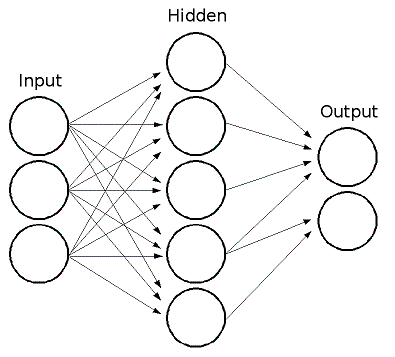
\includegraphics[width=80mm]{data/nn_simple.png}
\caption{El propòsit del layer \emph{hidden} s'explicarà més endavant.}
\label{simple_ann}
\end{figure}

La tasca principal d'una xarxa neuronal \emph{supervisada} és realitzar una \emph{aproximació de funció},
és a dir, a partir d'un seguit de valors de la funció (anomenat \emph{training set}), $ f(a) = b $, crear un model que s'ajusti a les dades
que se li ha subministrat \ref{func_approx} \autocite{msccsanad}. Podríem, per exemple, entrenar una \ac{ann} per a que realitzés
una aproximació de la funció $ sin(x)$, però és més interessant entrenar-la amb objectius més sofisticats; tot
problema determinista que es pugui reduir a \emph{produir unes sortides a partir d'uns valors d'entrada}, es pot
solucionar, molt probablement, amb una xarxa neuronal.

\begin{itemize}
\item \emph{Conduir un cotxe:} la posició, la velocitat, els cotxes adjacents, la carretera... una gran quantitat d'entrades. La nova direcció, 
accelerar o frenar, com a sortides.
\item \emph{Predir el flux del mercat de valors:} la pendent de la gràfica del valor d'una acció, els últims moviments, els últims compradors...
la xarxa s'ha entrenat amb dades històriques, i la història es repeteix. El moviment de l'accionista com a sortida.
\item \emph{Reconèixer caràcters:} aquesta és la nostra parada per a continuar amb l'explicació de les \ac{ann}. El conjunt de píxels que formen 
l'imatge d'un caràcter com a entrades, i el número que representen els píxels com a sortida. És un exemple fàcil d'aplicar i enriquidor.
\end{itemize}

El camí que segueix una \ac{ann} per a produir resultats és ben simple: els valors d'entrada passen per cada neurona a través d'una funció d'activació, regulada
pel valor anomenat pes, o \emph{weight} de la mateixa (literalment, és la importància que una determinada neurona
té en la xarxa completa. Les neurones amb pesos majors, realitzaran una aportació major al resultat de la xarxa neuronal). Tots els valors resultants d'un
layer es sumen de forma recursiva a cada neurona del layer següent, fins a arribar al final.

\begin{figure}[ht!]
\centering
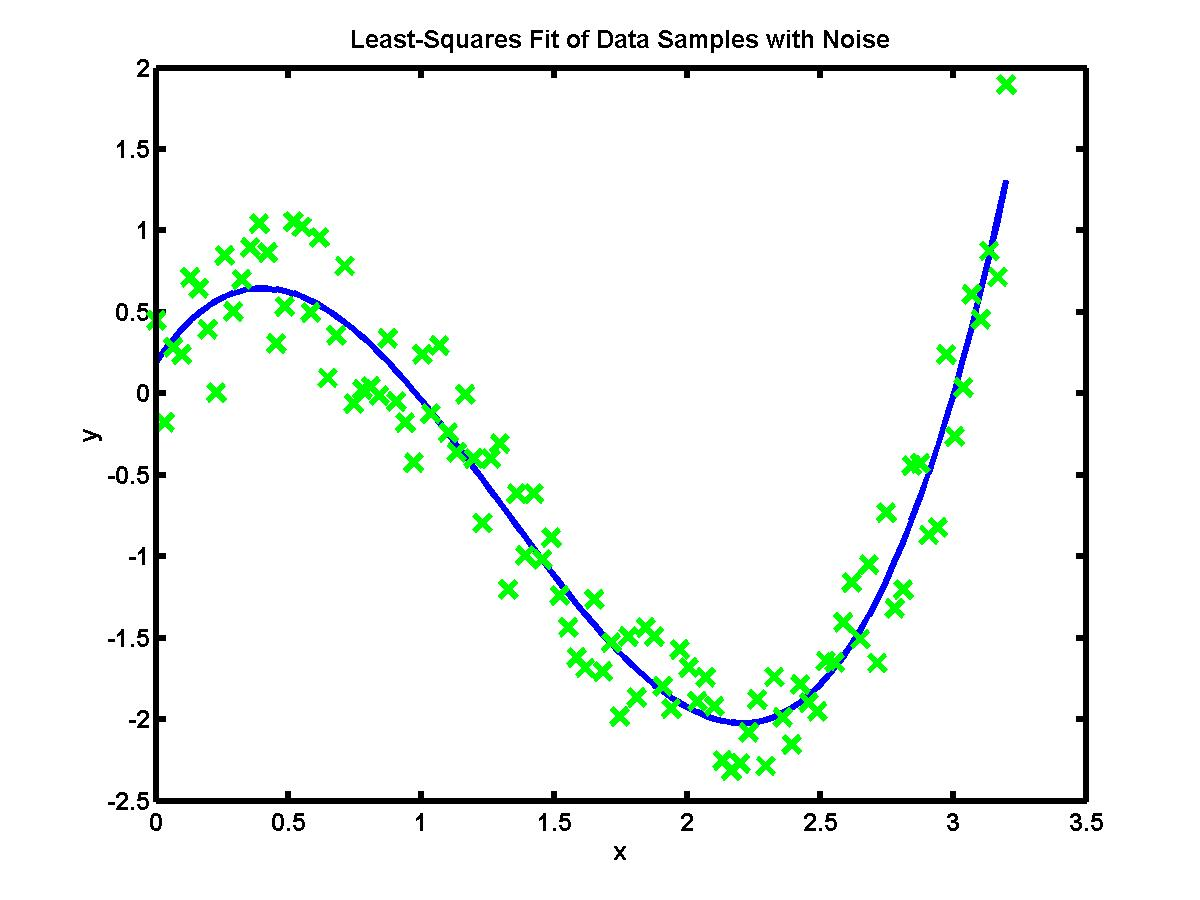
\includegraphics[width=80mm]{data/func_approx.jpg}
\caption{Exemple d'aproximació de funció. Els punts verds són els valors subministrats, el training set,
i la línia blava la funció que s'ha aproximat.}
\label{func_approx}
\end{figure}
